\newpage


\section{Projekt i wykonanie scrapera}\label{sec:projekt-scrapera}

Niniejszy rozdział poświęcono projektowi i wykonaniu scrapera - narzędzia służącego do automatycznego zbierania danych z sklepu internetowego tulski, omówionego w rozdziale~\ref{sec:projekt-platformy}.
Założono, że celem scrapera jest zgromadzenie informacji o wszystkich produktach dostępnych w sklepie internetowym, które mogą zostać wykorzystane do analizy asortymentu i cen produktów.
Kolejnym, istotnym założeniem rozdziału jest podejście typu czarnej skrzynki (ang. \emph{black-box})\cite{sekurak-testy-penetracyjne}.
Brak początkowej wiedzy na temat struktury i mechanizmów scrapowanego serwisu, jakim jest sklep internetowy tulski, nadaje realizm opisanym działaniom, odzwierciedlając warunki, w jakich najczęściej pracują osoby specjalizujące się w web scrapingu.
Poniższa część pracy jest zatem nie tylko technicznym studium przypadku, ale również wglądem w procesy myślowe i metody, które są wykorzystywane w realnych warunkach.

\subsection{Rekonesans}\label{subsec:rekonesans}

Rekonesans rozpoczął proces tworzenia scrapera, skupiając się na zrozumieniu celu, jakim jest sklep internetowy tulski.
Głównym zadaniem rekonesansu było zidentyfikowanie metod dających efektywny dostęp do interesujących danych.
Skupiono się na zrozumieniu mechanizmu ładowania i renderowania treści, strukturze zasobów oraz wykryciu potencjalnych wyzwań, które mogłyby wpłynąć na proces scrapowania.
Rekonesans jest kluczowym etapem w tworzeniu scrapera, ponieważ od niego zależą efektywność, awaryjność i stabilność narzędzia.
Przykładowo, jeśli podczas rekonesansu uda się znaleźć żądania API, które zwracają dane w formacie JSON, narzędzie będzie potencjalnie szybsze i bardziej odporne na zmiany.
Wynika to z faktu, że kontakt API zmienia się z reguły rzadziej niż interfejs graniczny użytkownika.

Kluczowym elementem rekonesansu była analiza ruchu sieciowego za pomocą narzędzi programistycznych wbudowanych w przeglądarkę internetową Firefox.
Po pierwsze, ustalono, że strona korzysta korzysta z proxy Cloudflare, co wskazuje nagłówek \emph{server} (patrz Listing~\ref{lst:rekonesans-get-homepage}).
Po drugie, odkryto, że strona została zbudowana z wykorzystaniem frameworka Next, co wskazuje nagłówek \emph{x-powered-by} (patrz listing~\ref{lst:rekonesans-get-homepage}).
Wykorzystanie Next oznacza wykorzystanie React, co może sugerować dynamiczne renderowanie treści.

\begin{listing}[H]
    \begin{minted}[xleftmargin=10pt,linenos,breaklines]{bash}
$ curl -I https://store.tulski.com
HTTP/2 200
date: Sun, 17 Dec 2023 17:09:05 GMT
content-type: text/html; charset=utf-8
cache-control: private, no-cache, no-store, max-age=0, must-revalidate
vary: RSC, Next-Router-State-Tree, Next-Router-Prefetch, Next-Url, Accept-Encoding
x-powered-by: Next.js
cf-cache-status: DYNAMIC
report-to: {"endpoints":[{"url":"https:\/\/a.nel.cloudflare.com\/report\/v3 ?s=l8mwfqVrt2h%2BXJYVshGNiHz%2FIRwSCEqIgVqxZ8kBhWWqkIGQaAuYiOy9 sv4JmNEGP1%2B53j1pVTVnm%2BpX2sID4%2BRDooubYk4tibHwMUz8sjuDxll1N rjXEffI6gReu1VJV7JI"}], "group":"cf-nel", "max_age":604800}
nel: {"success_fraction":0,"report_to":"cf-nel","max_age":604800}
server: cloudflare
cf-ray: 8370c5927feb666e-AMS
alt-svc: h3=":443"; ma=86400
    \end{minted}
    \caption{Nagłówki odpowiedzi dla strony domowej sklepu tulski}
    \label{lst:rekonesans-get-homepage}
\end{listing}

Po trzecie, w trakcie rekonesansu zauważono żądania do serwera API \emph{api.tulski.com}.
Odkrycie potwierdza hipotezę o dynamicznym renderowaniu treści na stronie.
Serwer API, podobnie jak witryna internetowa, korzysta z proxy Cloudflare.
Zidentyfikowano dwa żądania, które zwracają dane o produktach w formacie JSON\@.
Jednym z zidentyfikowanych żądań jest to, które zwraca listę produktów (zob. \autoref{fig:store-get-products-list}), wykorzystując paginację.
W żądaniu rozmiar strony jest określany parametrem \emph{limit}, a pozycję startową strony - parametrem \emph{offset}.

Przeprowadzono testy metodą prób i błędów, aby określić maksymalną liczbę produktów, jaką może zwrócić API w jednej odpowiedzi.
Ustalono, że parametr \emph{limit} nie posiada ścisłej walidacji, co umożliwia pobranie znacznie większej ilości danych niż to, co zwykle pobiera klient aplikacji internetowej.
Jednakże, zauważono, że ograniczeniem podczas pobierania dużej liczby rekordów jest czas otwarcia połączenia.
W przypadkach, gdy próbowano pobrać bardzo dużą liczbę rekordów, na przykład 8500 (zob. Listing~\ref{lst:store-get-products-list-8500}), serwer odpowiedział statusem \emph{504 Gateway Timeout}, wskazując na przekroczenie maksymalnego dopuszczalnego czasu przetwarzania żadania.
Maksymalną liczbą rekordów jaką udało się pobrać bez błędów było 8000 (zob. Listing~\ref{lst:store-get-products-list-8000}).


\begin{figure}[p]
    \begin{figure}[H]
        \centering
        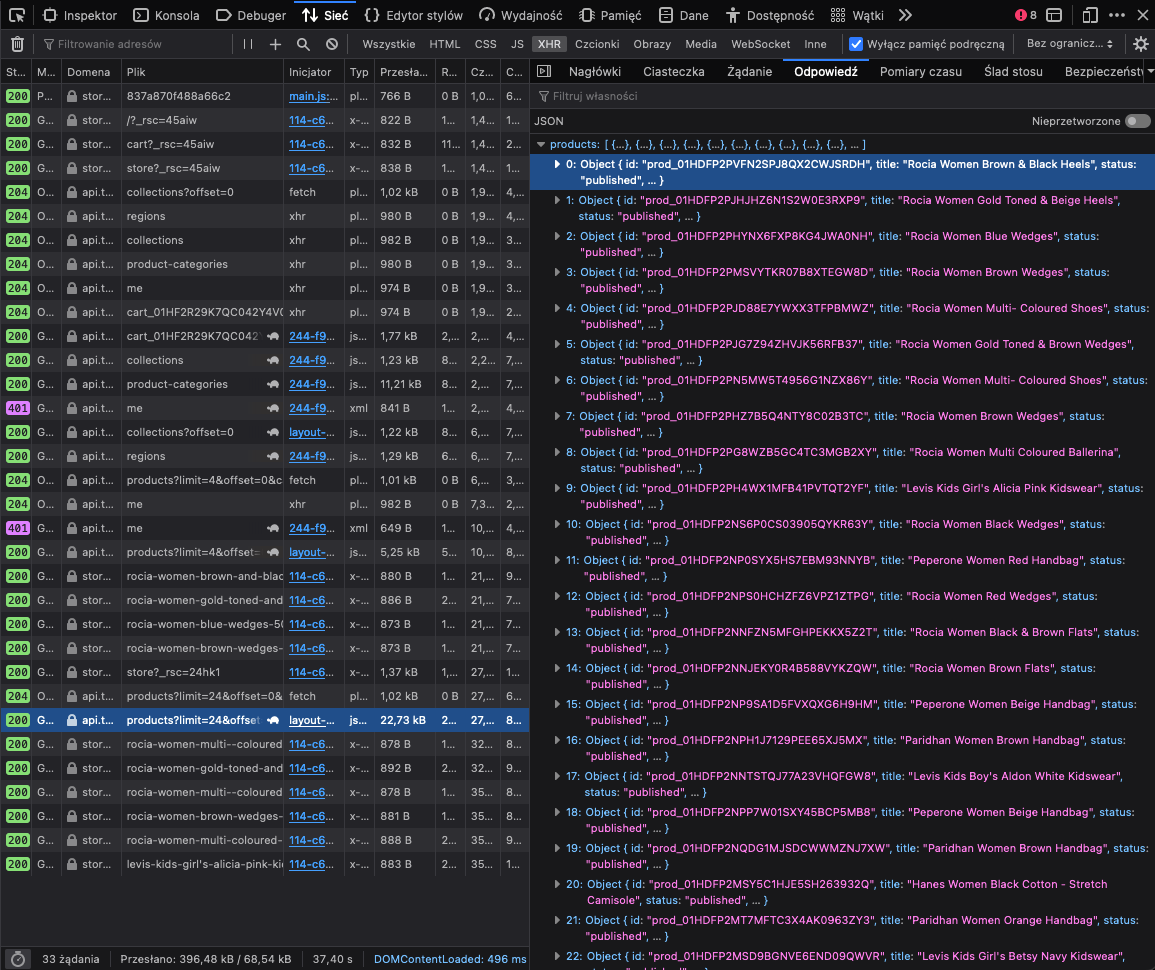
\includegraphics[width=0.8\textwidth]{img/store-get-products-list}
        \caption{Żądanie zwracające listę produktów}
        \label{fig:store-get-products-list}
    \end{figure}
    \begin{listing}[H]
        \begin{minted}[xleftmargin=10pt,linenos]{bash}
$ curl -X GET 'https://api.tulski.com/store/products?limit=8500' \
        -s \
        -o /dev/null \
        -w 'HTTP Code: %{http_code}\nTime Total: %{time_total}s\n'
HTTP Code: 504
Time Total: 61.691521s
        \end{minted}
        \caption{Żądanie 8500 produktów}
        \label{lst:store-get-products-list-8500}
    \end{listing}
    \begin{listing}[H]
        \begin{minted}[xleftmargin=10pt,linenos]{bash}
$ curl -X GET 'https://api.tulski.com/store/products?limit=8000' \
        -s \
        -o /dev/null \
        -w 'HTTP Code: %{http_code}\nTime Total: %{time_total}s\n'
HTTP Code: 200
Time Total: 60.223100s
        \end{minted}
        \caption{Żądanie 8000 produktów}
        \label{lst:store-get-products-list-8000}
    \end{listing}
\end{figure}

\newpage

Następne żądanie API, które zwróciło uwagę podczas rekonesansu, dotyczyło pobierania szczegółowych danych o produkcie (zob. \autoref{fig:store-get-product-details}).
Odpowiedź serwera na to żądanie zawiera bogaty zestaw danych o produkcie, w tym nazwę, opis, zdjęcia, linki do obrazów, metadane oraz szczegóły dotyczące rozmiarów i wariantów z ich dostępności.
Struktura danych w formacie JSON, wykorzystana w odpowiedzi (zob. Listing ~\autoref{lst:store-get-product-details-request}), jest przejrzysta i dobrze zorganizowana.
Zwracane dane wyczerpują wymagania postawione przed scraperem.

\begin{figure}[H]
    \centering
    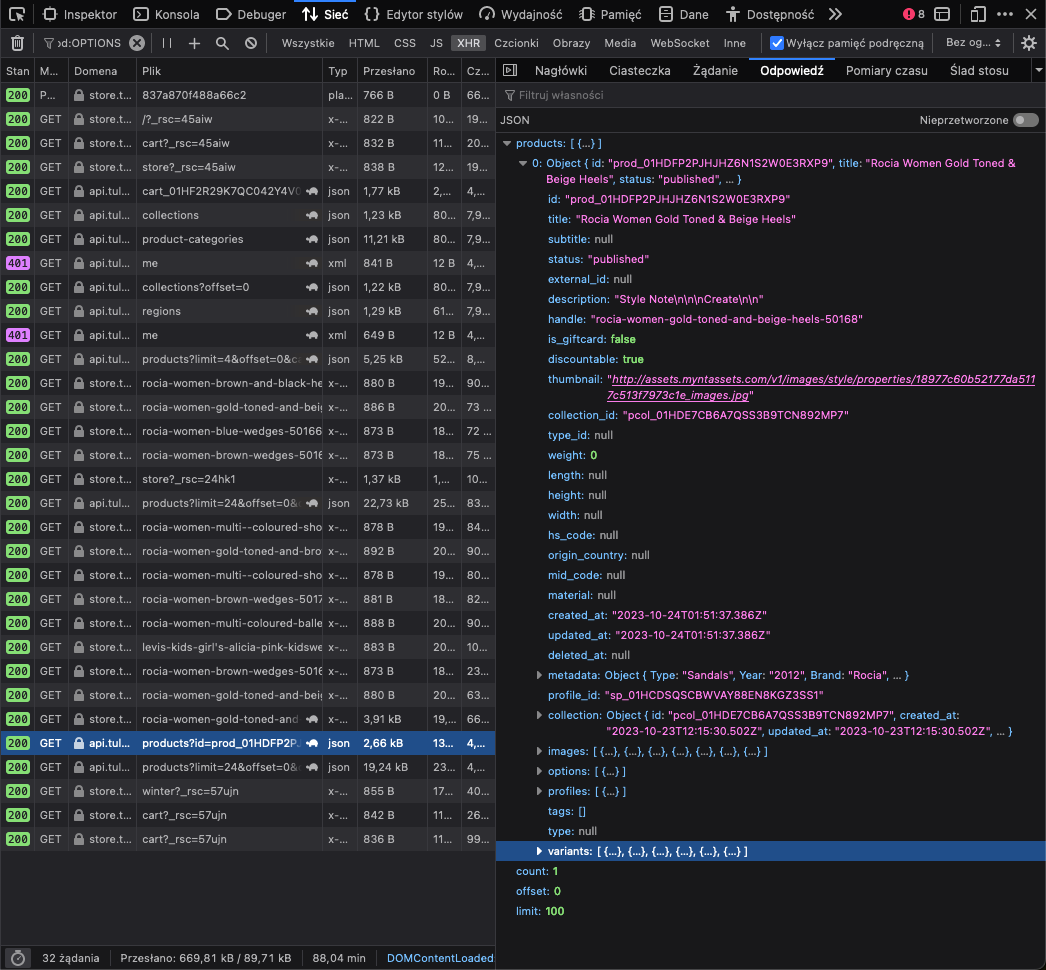
\includegraphics[width=0.8\textwidth]{img/store-get-product-details}
    \caption{Żądanie po szczegóły produktu}
    \label{fig:store-get-product-details}
\end{figure}
\begin{listing}[H]
    \begin{minted}[xleftmargin=10pt,linenos,breaklines]{bash}
$ curl -G -d "id=prod_01HDFP2PJHJHZ6N1S2W0E3RXP9" \
        "https://api.tulski.com/store/products"
{"products": [{"id": "prod_01HDFP2PJHJHZ6N1S2W0E3RXP9", "title": "Rocia Women Gold Toned & Beige Heels", "subtitle": null, "status": "published", "external_id": null, "description": "Style Note\n\n\nCreate\n\n", "handle": "rocia-women-gold-toned-and-beige-heels-50168", "is_giftcard": false, "discountable": true, "thumbnail": ...
    \end{minted}
    \caption{Struktura JSON odpowiedzi na żądanie po szczegóły produktu}
    \label{lst:store-get-product-details-request}
\end{listing}


\subsection{Implementacja}\label{subsec:scraper-implementation}

Po uzyskaniu odpowiedniej ilości danych w trakcie rekonesansu, rozpoczęto proces tworzenia scrapera.
Wykorzystano język TypeScript (zob. \autoref{subsec:typescript}), środowisko uruchomieniowe Node.js (zob. \autoref{subsec:nodejs}) i bibliotekę got (zob. \autoref{subsec:got}).

\noindent\textbf{Konfiguracja klienta HTTP}

Skonfigurowano klienta HTTP \url{storeClient}, który wysyła żądania do serwera API z nagłówki typowymi dla przeglądarki internetowej.
Działanie to miało na celu jak najwierniejsze odwzorowanie śladu i zachowań scrapera na wzór klienta przeglądarkowego, co zwiększa jego dyskrecję podczas działania.
Ponadto dodano logowanie żądań i odpowiedzi, co znacząco ułatwia proces debugowania, monitorowania i identyfikacji potencjalnych błędów.
Konfiguracja została przedstawiona na Listingu~\ref{lst:store-http-client-config}.

\begin{listing}[H]
    \begin{minted}[xleftmargin=10pt,linenos,breaklines]{typescript}
const storeClient: typeof got = got.extend({
  prefixUrl: "https://api.tulski.com/",
  hooks: {
    beforeRequest: [requestLogger(logger)],
    afterResponse: [responseLogger(logger)],
  },
  headers: {
    "User-Agent":
      "Mozilla/5.0 (Macintosh; Intel Mac OS X 10.15; rv:121.0) Gecko/20100101 Firefox/121.0",
    Accept: "*/*",
    "Accept-Language": "en-US,en;q=0.7,pl;q=0.3",
    "Accept-Encoding": "gzip, deflate, br",
    "Access-Control-Request-Method": "GET",
    DNT: "1",
    "Sec-GPC": "1",
    Connection: "keep-alive",
    "Sec-Fetch-Dest": "empty",
    "Sec-Fetch-Mode": "cors",
    "Sec-Fetch-Site": "same-site",
    Pragma: "no-cache",
    "Cache-Control": "no-cache",
  },
});
    \end{minted}
    \caption{Konfiguracja klienta HTTP storeClient}
    \label{lst:store-http-client-config}
\end{listing}

\noindent\textbf{Funkcja pobierająca listę produktów}

Następnie, zaimplementowano funkcje \mintinline{text}{getProductsList} służącą do pobierania listy produktów (zob. Listing~\ref{lst:store-http-client-getProductsList}).
Wykorzystano Pagination API biblioteki got\cite{got-paginate-docs}, które pozwala na iteracyjne pobieranie kolejnych pozycji z listy.
Funkcja \mintinline{text}{transform} parsuje otrzymaną odpowiedź w formacie JSON do tablicy produktów.
Następnie funkcja paginate, wylicza parametry dla kolejnych stron, wykorzystując aktualną długość listy produktów i parametr offset.

\begin{listing}[p]
    \begin{minted}[xleftmargin=10pt,linenos,breaklines]{typescript}
export const getProductsList = () => {
  return storeClient.paginate({
    url: "/store/products",
    searchParams: {
      currency_code: "eur",
      is_giftcard: false,
    },
    pagination: {
      transform: (response: Response<string>): ProductListing[] => {
        return JSON.parse(response.body).products;
      },
      paginate: ({ response, currentItems }) => {
        if (currentItems.length === 0) {
          return false;
        }
        const searchParams = response.request.options
          .searchParams as URLSearchParams;
        const previousOffset = Number(searchParams?.get("offset") ?? 0);
        return {
          searchParams: {
            offset: previousOffset + currentItems.length,
          },
        };
      },
      countLimit: 5000,
      // Wait before making another request to prevent API rate limiting.
      backoff: 500,
      // It is a good practice to set an upper limit of how many requests can be made.
      // This way we can avoid infinite loops.
      requestLimit: 1000,
      // In this case, we don't need to store all the items we receive.
      // They are processed immediately.
      stackAllItems: false,
    },
  });
};
    \end{minted}
    \caption{Funkcja pobierająca listę produktów}
    \label{lst:store-http-client-getProductsList}
\end{listing}

\noindent\textbf{Funkcja pobierająca szczegóły produktu}

Kolejna funkcja, \mintinline{text}{getProductDetails}, służy do pobierania szczegółowych danych o konkretnym produkcie na podstawie jego identyfikatora.
Wykorzystano metodę \mintinline{text}{get} biblioteki got.

\begin{listing}[H]
    \begin{minted}[xleftmargin=10pt,linenos,breaklines]{typescript}
export const getProductDetails = (
  productId: string,
): CancelableRequest<ProductResponse> => {
  return storeClient
    .get(`/store/products/${productId}`, {
      searchParams: {
        currency_code: "eur",
      },
    })
    .json();
};
    \end{minted}
    \caption{Funkcja pobierająca szczegóły produktu}
    \label{lst:store-http-client-getProductDetails}
\end{listing}

